\begin{figure}
	\centering
	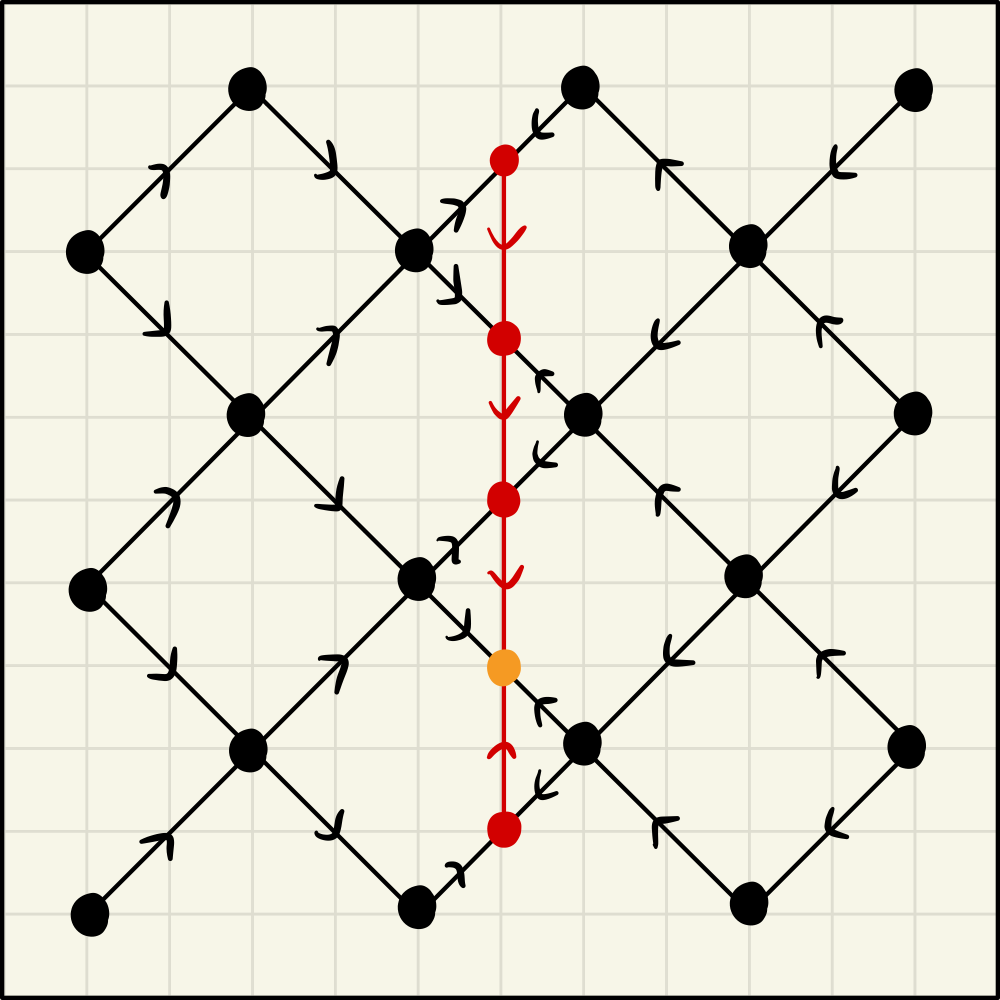
\includegraphics[width=0.6\textwidth]{figures/Tensor_Networks/disoTPS.jpeg}
	\caption{A diagonal isometric tensor network on a square lattice is constructed from site tensors $T_i$ (drawn in black) and an orthogonality hypersurface of auxillary tensors $W_i$ (drawn in red). The orthogonality hypersurface is rotated by $45^\circ$ with respect to the lattice.}
	\label{fig:disoTPS_structure}
\end{figure}
The structure of a disoTPS on a square lattice is shown in figure \figref{fig:disoTPS_structure}. It can be constructed in three steps. First, a square PEPS is rotated by $45^\circ$. Next, the orthogonality hypersurface is constructed as a column of auxillary tensors. The auxillary tensors are connected in a line similar to an MPS and placed between between two columns of PEPS tensors. Note that, in contrast to the standard isoTPS the tensors of the orthogonality hypersurface do not carry any physical degrees of freedom and are only connected via virtual bonds to the neighboring tensors. Lastly, the isometry condition is enforced such that all arrows point towards the orthogonality hypersurface. Tensors left of the orthogonality surface are thus brought into a left-isometric form and tensors right of the orthogonality surface are brought into a right-isometric form, as shown in figure \figref{fig:disoTPS_structure}. The auxillary tensors making up the orthogonality hypersurface are isometrized such that all arrows point towards a single auxillary tensor, the orthogonality center. \par
In the following, we will denote the auxillary tensors by $W_i$, and the tensors carrying physical degrees of freedom with $T_i$. The bonds connecting two $T$-tensors or a $T$-tensor and a $W$-tensor are truncated to a maximal bond dimension of $D$, while the maximal bond dimension between two $W$-tensors is denoted as $\chi$. In practice it is found that setting $\chi=f\cdot D$ with an integer $f\ge1$ produces good results. \par
Similar to the standard isoTPS, the orthogonality center can easily and exactly be moved along the orthogonality hypersurface using QR-decompositions. Moving the orthogonality hypersurface to the left or to the right is a harder problem and will be discussed in section \ref{sec:disoTPS_yang_baxter_move}. \par
\begin{figure}
	\centering
	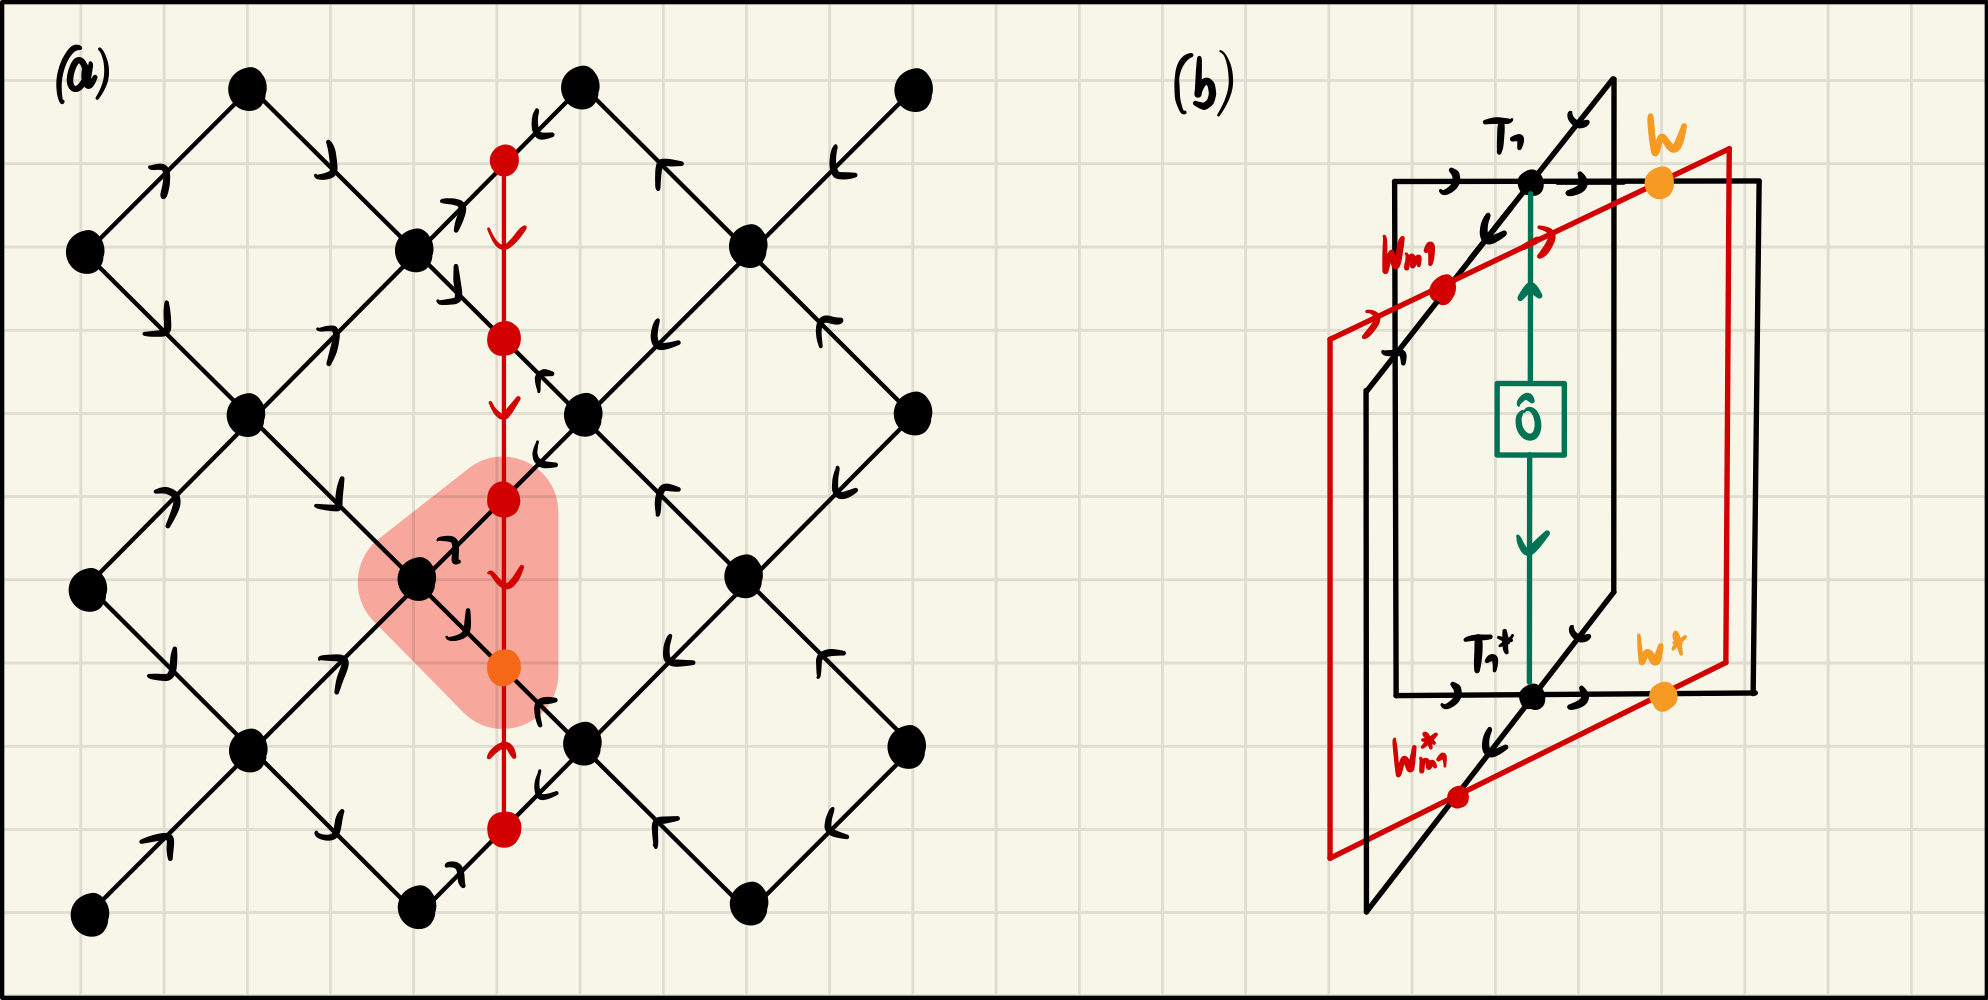
\includegraphics[width=0.9\textwidth]{figures/Tensor_Networks/disoTPS_onesite_expectation_value.jpeg}
	\caption{(a) The one-site wavefunction around a site $i$ is the sub network containing the site tensor $T_i$ and the two connected auxillary tensors. (b) Computation of a single site expectation value reduces to the shown contraction over a one-site wavefunction, its complex conjugate, and the one-site operator $\hat{O}_i$.}
	\label{fig:disoTPS_onesite_expectation_value}
\end{figure}
As in MPS and standard isoTPS, disoTPS allow for the fast computation of expectation values of local operators. The expectation value $\left\langle\Psi\right|\hat{O}_i\left|\Psi\right\rangle$ of a one-site operator $\hat{O}_i$ acting on site $i$ can be computed as follows: First, the orthogonality center is moved next to site $i$. We next define the \textit{one-site wavefunction} as the sub-network containing the site tensor $T_i$ and the two connected $W$-tensors. Note that the one-site wavefunction is connected to its environment only by bonds with incoming arrows. Next the wavefunction is contracted with its complex conjugate, sandwhiching the operator $\hat{O}_i$ between the two. Due to the isometry condition, this reduces to a contraction of only the one-site wavefunction, its complex conjugate, and the operator $\hat{O}_i$, as shown in figure \ref{fig:disoTPS_onesite_expectation_value}. This contraction has a computational cost scaling as $\mathcal{O}\left(\chi^3 D^3 + D^6d^2\right)$ and gives as result the desired expectation value. \par
\begin{figure}
	\centering
	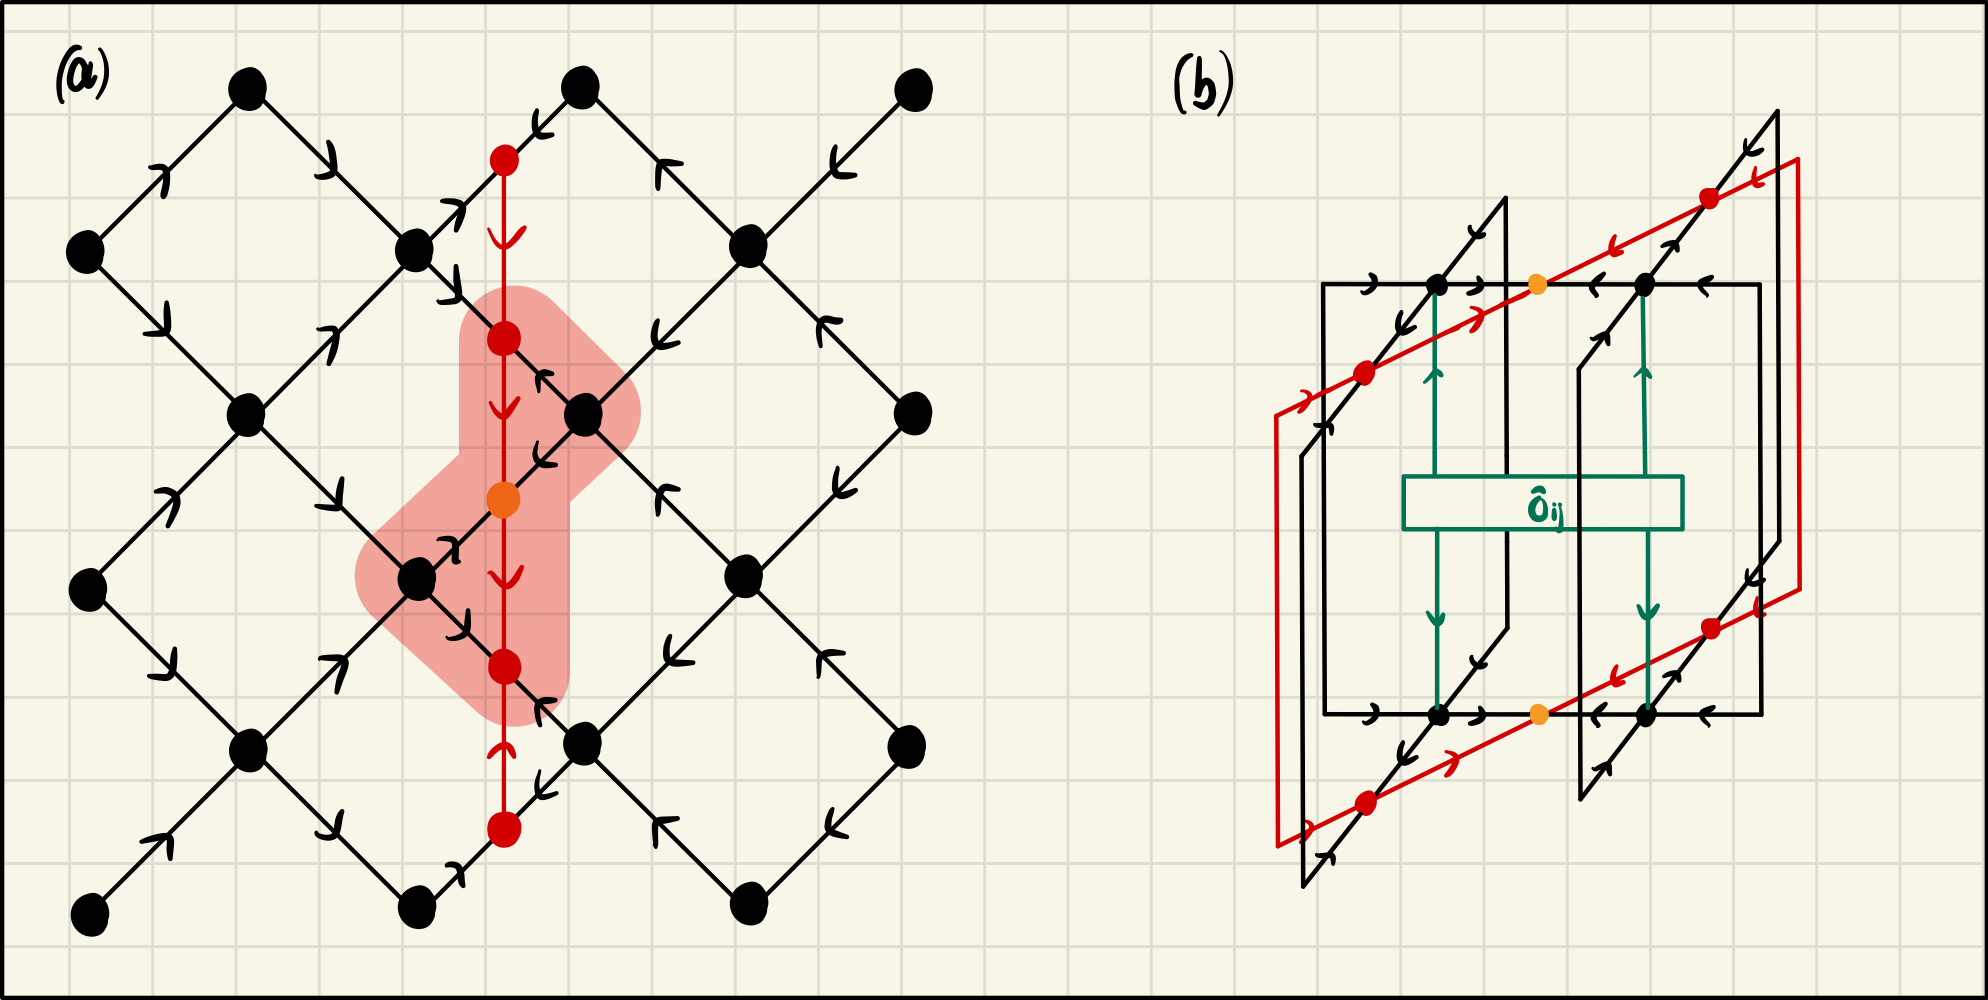
\includegraphics[width=0.9\textwidth]{figures/Tensor_Networks/disoTPS_twosite_expectation_value.jpeg}
	\caption{(a) The two-site wavefunction around neighboring sites $i$ and $j$ is the sub network containing the site tensors $T_i$ and $T_j$ and the three connected auxillary tensors. (b) Computation of a two-site expectation value reduces to the shown contraction over a two-site wavefunction, its complex conjugate, and the two-site operator $\hat{O}_{ij}$.}
	\label{fig:disoTPS_twosite_expectation_value}
\end{figure}
The expectation value $\left\langle\Psi\right|\hat{O}_{ij}\left|\Psi\right\rangle$ of a two-site operator $\hat{O}_{ij}$ acting on two neighbouring sites $i$ and $j$, also called \textit{bond operator}, can be computed similarly. First, the orthogonality center is moved such that it sits in the middle of the bond connecting sites $i$ and $j$. The \textit{two-site wavefunction} is then defined as the subnetwork containing the two site tensors $T_i$ and $T_j$ and three $W$-tensors as shown in figure \ref{fig:disoTPS_twosite_expectation_value}, such that again all legs connecting the subnetwork to its environment are only decorated with arrows pointing towards the two-site wavefunction. The computation of the expectation value then reduces to the contraction of only the two-site wavefunction with its complex conjugate and the bond operator $\hat{O}_{ij}$. The computational cost of this contraction scales as $\mathcal{O}\left(\chi^3D^3d^2\right)$.